\documentclass[a4paper,12pt]{article}

% Use the Classic Thesis style
%
% \usepackage[nochapters]{classicthesis}

\usepackage[T1]{fontenc}
\usepackage[utf8]{inputenc}

% Use text fonts
%
\usepackage{lmodern}  % the Latin Modern fonts which is an enhanced version of the Computer Modern fonts
% \usepackage{tgschola}  % the Gyre Schola fonts which is an enhanced version of the New Centrury Schoolbook fonts

% Use math fonts
%
% \usepackage{concmath}  % the Concrete Math fonts
% \usepackage{euler}  % the Euler Math fonts
% \usepackage{kerkis}  % the Kerkis fonts

% Some font packages that provide math font may override the text font, the
% following three commands reset it to the default.
%
% For the Latin Modern fonts
%
% \renewcommand{\rmdefault}{lmr}
% \renewcommand{\sfdefault}{lmss}
% \renewcommand{\ttdefault}{lmtt}
%
% For the Gyre Schola fonts
%
% \renewcommand{\rmdefault}{qcs}

\usepackage{amsmath}

% Use the MH bundle
%
% \usepackage{mhsetup}
% \usepackage{mathtools}
% \usepackage{mathstyle}
% \usepackage{breqn}
% \usepackage{empheq}
% \usepackage{flexisym}

% Use AMS-style theorem
%
\usepackage{amsthm}
% \theoremstyle{definition}
% \newtheorem{theorem}{Theorem}

% Use MATH formulas in PARagraph mode Typesetting Inference Rules
% 
\usepackage{mathpartir}

\usepackage{tikz}
\usepackage{tikz-qtree}
\usepackage{bigfoot}

% New commands
%
\newcommand{\term}[1]{\textsf{#1}}
\newcommand{\appl}[2]{#1\inparens{#2}}
\newcommand{\eval}[2]{#1 \Longrightarrow #2}
\newcommand{\redc}[2]{#1 \longrightarrow #2}

\usepackage{stmaryrd}  % the St Mary’s Road symbol font


\newcommand{\atangles}[1]{\langle#1\rangle}
\newcommand{\atparens}[1]{(#1)}
\newcommand{\atbracks}[1]{[#1]}
\newcommand{\atbraces}[1]{\{#1\}}
\newcommand{\atfloors}[1]{\lfloor#1\rfloor}
\newcommand{\atceils}[1]{\lceil#1\rceil}
\newcommand{\atucorners}[1]{\ulcorner#1\urcorner}
\newcommand{\atlcorners}[1]{\llcorner#1\lrcorner}
\newcommand{\atlparens}[1]{\llparenthesis#1\rrparenthesis}
\newcommand{\atlbracks}[1]{\llbracket#1\rrbracket}
\newcommand{\atbars}[1]{|#1|}
\newcommand{\atbbars}[1]{\|#1\|}

\newcommand{\inangles}[1]{\langle#1\rangle}
\newcommand{\inparens}[1]{\left(#1\right)}
\newcommand{\inbracks}[1]{\left[#1\right]}
\newcommand{\inbraces}[1]{\left\{#1\right\}}
\newcommand{\infloors}[1]{\left\lfloor#1\right\rfloor}
\newcommand{\inceils}[1]{\left\lceil#1\right\rceil}
\newcommand{\inucorners}[1]{\left\ulcorner#1\right\urcorner}
\newcommand{\inlcorners}[1]{\left\llcorner#1\right\lrcorner}
\newcommand{\inlparens}[1]{\left\llparenthesis#1\right\rrparenthesis}
\newcommand{\inlbracks}[1]{\left\llbracket#1\right\rrbracket}
\newcommand{\inbars}[1]{\left|#1\left|}
\newcommand{\inbbars}[1]{\left\|#1\right\|}

\newcommand{\texterr}[1]{\textcolor{red}{#1}}

\newenvironment{grammar}
 {\begin{center}\small\begin{tabular}{rrclr}}
 {\end{tabular}\normalsize\end{center}}
\newcommand{\prodhead}[5]{#1 & #2 & #3 & #4 & #5 \\}
\newcommand{\prodrule}[3]{      & & #1 & #2 & #3 \\}



% Front elements
%
\title{
 Programming Languages and Types \\~\\
 \textbf{Exercise 10}
}
\author{
 Yi Dai
}

\begin{document}

\maketitle

\section{Concrete Syntax and Abstract Syntax}

The following BNF grammar defines the \term{concrete syntax} of a language for (a subset
of) arithmetic expressions (thus call the language AE).

\begin{grammar}
 \prodhead{(expression)}{$Exp$}{::=}{$Nat$}{(number)}
 \prodrule{|}{$Exp\ Opr\ Exp$}{(compound)}
 \\
 \prodhead{(operator)}{$Opr$}{::=}{\tt +}{(plus)}
 \prodrule{|}{\tt -}{(minus)}
 \prodrule{|}{\tt *}{(times)}
 \prodrule{|}{\tt /}{(divides)}
\end{grammar}

From $Exp$, we can derive all valid \term{parse trees} of AE.  For example, the following
two trees could be derived.

\begin{center}
 \begin{tabular}{c c}
  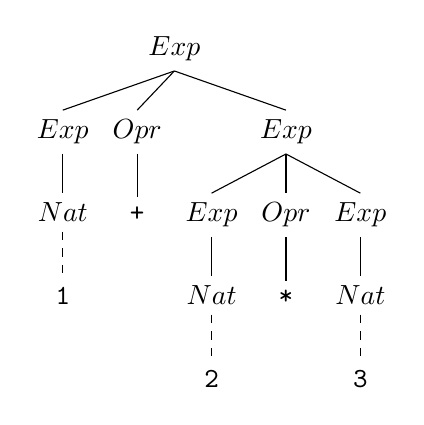
\begin{tikzpicture}
   \Tree [ .$Exp$ [ .$Exp$ [ .$Nat$ \edge[dashed]; {\tt 1} ] ]
                  [ .$Opr$ {\tt +} ]
                  [ .$Exp$ [ .$Exp$ [ .$Nat$ \edge[dashed]; {\tt 2} ] ]
                           [ .$Opr$ {\tt *} ]
                           [ .$Exp$ [ .$Nat$ \edge[dashed]; {\tt 3} ] ] ] ] ]
  \end{tikzpicture}
  &
  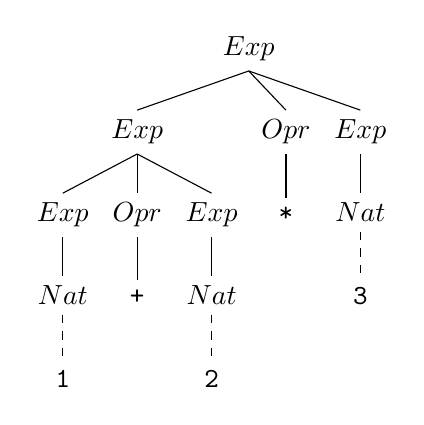
\begin{tikzpicture}
   \Tree [ .$Exp$ [ .$Exp$ [ .$Exp$ [ .$Nat$ \edge[dashed]; {\tt 1} ] ]
                           [ .$Opr$ {\tt +} ]
                           [ .$Exp$ [ .$Nat$ \edge[dashed]; {\tt 2} ] ] ]
                  [ .$Opr$ {\tt *} ]
                  [ .$Exp$ [ .$Nat$ \edge[dashed]; {\tt 3} ] ] ]
  \end{tikzpicture}
 \end{tabular}
\end{center}

However, only one \emph{string} of symbols, namely \verb|1 + 2 * 3|, can be read out
from left to right.  The string is supposed to encode the tree.  But obviously, it
fails to include into the encoding the part that structurally differs one from the
other.  The distinguishing part indicates whether it is \verb|2 * 3| or \verb|1 + 2|
that should be first evaluated, hence $7$ or $9$ that should be assigned to the tree.
Since \verb|1 + 2 * 3| leves out this important information, it is \emph{ambiguous}.
On one hand, when you \emph{write} it, you could not make clear which tree you intend
and what you mean; on the other hand, when I \emph{read} it, I could not make sure
which tree is intended and what is meant.

This suggests that the above grammar is \emph{adequate} for \emph{specifying} all the
\emph{structures} of the language (from it we can derive all valid parse trees), but
is \emph{inadequate} for \emph{determining} the structure encoded in a string
(following it we can not build a unique parse tree for some strings).  The grammar is
said to be \emph{ambiguous}.  To remove the ambiguity, the grammar must be enriched.
The following improved grammar is no longer ambiguous.

\begin{grammar}
 \prodhead{(level-0 expression)}{$Exp$}{::=}{$Exp_1$}{(level-1 expression)}
 \prodrule{|}{$Exp\ LOp\ Exp_1$}{(level-0 compound)}
 \\
 \prodhead{(level-1 expression)}{$Exp_1$}{::=}{$Exp_2$}{(leve-2 expression)}
 \prodrule{|}{$Exp_1\ HOp\ Exp_2$}{(level-1 compound)}
 \\
 \prodhead{(level-2 expression)}{$Exp_2$}{::=}{$Nat$}{(number)}
 \prodrule{|}{\tt ( $Exp$ )}{(parenthesized)}
 \\
 \prodhead{(lower operator)}{$LOp$}{::=}{$+$}{(plus)}
 \prodrule{|}{$-$}{(minus)}
 \\
 \prodhead{(lower operator)}{$LOp$}{::=}{$*$}{(times)}
 \prodrule{|}{$/$}{(divides)}
\end{grammar}

It classifies the operators into two groups, one ($LOp$) of lower precedence and the
other ($HOp$) of higher precedence, and divides the expressions accordingly into three
levels, from level 0 ($Exp$, with the subscript $0$ omitted) with lowest priority through
level 2 ($Exp_2$) with highest priority.  So in an expression, sub-expressions in level-2
will first be evaluated, then level-1 sub-expressions, and finally level-0.
Sub-expressions in the same level are evaluated from left to right.  Strictly speaking,
parentheses can solve the problem, however, operator precedence and associativity allows
us to still write \verb|1 + 2 * 3| instead of \verb|1 + (2 * 3)| (which results a more
complicated parse tree) to mean $7$.  With the new grammar, the string \verb|1 + 2 * 3|
encodes only the following tree:

\begin{center}
 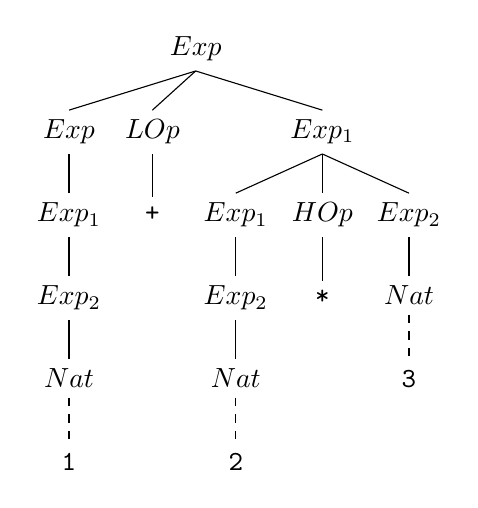
\begin{tikzpicture}
  \Tree [ .$Exp$ [ .$Exp$ [ .$Exp_1$ [ .$Exp_2$ [ .$Nat$ \edge[dashed]; {\tt 1} ] ] ] ]
                 [ .$LOp$ {\tt +} ]
                 [ .$Exp_1$ [ .$Exp_1$ [ .$Exp_2$ [ .$Nat$ \edge[dashed]; {\tt 2} ] ] ]
                           [ .$HOp$ {\tt *} ]
                           [ .$Exp_2$ [ .$Nat$ \edge[dashed]; {\tt 3} ] ] ] ] ]
 \end{tikzpicture}
\end{center}

Instead, the tree as follows would gain the meaning $9$ and is encoded by the string
\verb|(1 + 2) * 3|.

\begin{center}
 \begin{tikzpicture}
  \Tree [ .$Exp$
           [ .$Exp_1$
              [ .$Exp_1$
                 [ .$Exp_2$
                    [ {\tt (}
                      [ .$Exp$ 
                         [ .$Exp$
                            [ .$Exp_1$
                               [ .$Exp_2$ [ .$Nat$ \edge[dashed]; {\tt 1} ] ] ] ]
                         [ .$LOp$ {\tt +} ]
                         [ .$Exp_1$ [ .$Exp_2$ [ .$Nat$ \edge[dashed]; {\tt 2} ] ] ] ]
                      {\tt )} ] ] ]
              [ .$HOp$ {\tt *} ]
              [ .$Exp_2$ [ .$Nat$ \edge[dashed]; {\tt 3} ] ] ] ]
 \end{tikzpicture}
\end{center}

Whether the grammar is ambiguous or not, we see that parse trees for simple arithmetic
expressions are very complicated, especially those obtained from the unambiguous grammar.
Moreover, this complication does not contribute much to the meaning of the expression.
Instead, it buries the structure that is \emph{essential} for us to decide the meaning
for an expression.  For example, the essential structure of the parse tree for
\verb|1 + 2 * 3| is simply
\begin{center}
 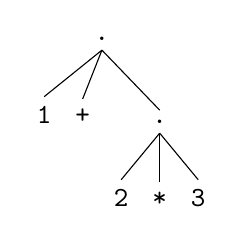
\begin{tikzpicture}
  \Tree [ .{\tt .} {\tt 1} {\tt +} [ .{\tt .} {\tt 2} {\tt *} {\tt 3} ] ]
 \end{tikzpicture}
\end{center}
and for \verb|(1 + 2) * 3|
\begin{center}
 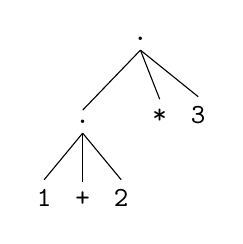
\begin{tikzpicture}
  \Tree [ .{\tt .} [ .{\tt .} {\tt 1} {\tt +} {\tt 2} ] {\tt *} {\tt 3} ]
 \end{tikzpicture}
\end{center}
That is to say, unambiguous concrete syntax is important when we want to write actual
programs in it, but for semantic analysis of the language, only structures matter.
Thus a grammar will serve us well as long as it covers all the structures of the
language.  Whether it is ambiguous or not is a secondary matter.  Such a grammar for
AE is given below:
\begin{gather*}
 e \in Exp \\
 n \in Nat \\
 o \in Opr
\end{gather*}
\begin{grammar}
 \prodhead{(expression)}{$e$}{::=}{$n$}{(number)}
 \prodrule{|}{$e_1\ o\ e_2$}{(compound)}
 \\
 \prodhead{(operator)}{$o$}{::=}{\tt +}{(plus)}
 \prodrule{|}{\tt -}{(minus)}
 \prodrule{|}{\tt *}{(times)}
 \prodrule{|}{\tt /}{(divides)}
\end{grammar}

A form like $e \in Exp$ says that the meta-variable (variable in our meta-language,
English and mathematics) $e$ can range over the set $Exp$ of expressions.  The
specifications for the \term{syntactic category} expression and operator reuses the
BNF notation.  It specifies that the possible structure of AE is one of the following:
\begin{center}
 \begin{tabular}{c c}
  \begin{tikzpicture}
   \Tree [ .$n$ ]
  \end{tikzpicture}
  &
  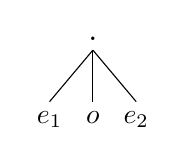
\begin{tikzpicture}
   \Tree [ .{\tt .} $e_1$ $o$ $e_2$ ]
  \end{tikzpicture}
 \end{tabular}
\end{center}
That is, it can be either a number or a compound expression.

\begin{verbatim}
sealed abstract class Exp
type Opr = String
case class Num(int : Int) extends Exp
case class Cpd(opr : Opr, lhs : Exp, rhs : Exp) extends Exp
\end{verbatim}

\noindent
It would be ideal to write programs directly by drawing their abstract syntax trees.
But normally we write programs in text as \emph{strings} of symbols.  These strings
encode the structures and they form a language.  So a language definition
\emph{assigns} strings to structures.  Such a definition can be given by a set of
grammar production rules.

\subsection{Specification vs. Identification}

The grammar

\begin{grammar}
 \prodhead{(expression)}{$Exp$}{::=}{$Int$}{(number)}
 \prodrule{|}{$Exp\ Opr\ Exp$}{(compound)}
 \\
 \prodhead{(operator)}{$Opr$}{::=}{\tt +}{(plus)}
 \prodrule{|}{\tt -}{(minus)}
 \prodrule{|}{\tt *}{(times)}
 \prodrule{|}{\tt /}{(divides)}
\end{grammar}

\noindent
defines a language for arithmetic expressions.  For every structure, this grammar can
generate a \emph{unique} expression that encodes the structure.  For example, for the
following two tree structures
\begin{center}
 \begin{tabular}{c c}
  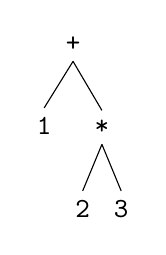
\begin{tikzpicture}
   \Tree [ .{\tt +} {\tt 1}
                    [ .{\tt *} {\tt 2} {\tt 3} ] ]
  \end{tikzpicture}
  &
  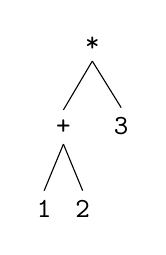
\begin{tikzpicture}
   \Tree [ .{\tt *} [ .{\tt +} {\tt 1} {\tt 2} ]
                    {\tt 3} ]
  \end{tikzpicture}
 \end{tabular}
\end{center}
it will generate the expression \verb|1 + 2 * 3|.  This encoding loses some information,
namely the structural differences between the two tree structures.  So the grammar is
\emph{inadequate} to be used in the inverse direction.  Since given the expression to it.
\verb|1 + 2 * 3|, we cannot decide which tree structure of the two above to assign
In turn, we cannot decide which meaning to assign to it, since the two tree structures
means differently: one 7, the other 9.  In other words, the expression \verb|1 + 2 * 3|
is \emph{ambiguous}.  One way to avoid this ambiguity is by adding parentheses to the
grammar:
\begin{grammar}
 \prodhead{(expression)}{$Exp$}{::=}{$\ldots$}{}
 \prodrule{|}{{\tt (}\ $Exp$\ {\tt )}}{(parenthesized)}
\end{grammar}
Whenever there exists ambiguity, add parentheses.  Now two expressions \verb|1 + (2 * 3)|
and \verb|(1 + 2) * 3| can be assigned to the two trees above respectively.  At this point,
the grammar is adequate for \emph{theoretical} discussion about the semantics of the
expressions in the language.  It can also be used inversely to identify the structure
associated to an expression.  However, in \emph{paractice}, one always wants to write
programs more concisely, say, using as few parentheses as possible.

\emph{specifies} all possible \emph{tree structures} of arithmetic expressions.  It
can be used to generate all possible arithmetic expressions (represented as strings
of symbols), but it \emph{cannot} be used to \emph{identify} the tree structure
associated to an arithmetic expression.  For example, the grammar can produce the
arithmetic expression \verb|1 + 2 * 3|, but given this expression, it cannot figure
out what the expression is intended to notate, the tree structure associated to
\verb|(1 + 2) * 3| or the tree associated to \verb|1 + (2 * 3)|.  In other words,
the notation \verb|1 + 2 * 3| is ambiguous.  To overcome this problem the following
more complicated grammar has to be used.

\begin{grammar}
 \prodhead{(level-0 expression)}{$Exp$}{::=}{$Exp_1$}{(level-1 expression)}
 \prodrule{|}{$Exp\ LOp\ Exp_1$}{(compound level 1)}
 \\
 \prodhead{(level-1 expression)}{$Exp_1$}{::=}{$Exp_2$}{(level-2 expression)}
 \prodrule{|}{$Exp_1\ HOp\ Exp_2$}{(compound level 2)}
 \\
 \prodhead{(level-2 expression)}{$Exp_2$}{::=}{$Int$}{(number)}
 \prodrule{|}{$\inparens{\ Exp\ }$}{(parenthesized)}
 \\
 \prodhead{(lower operator)}{$LOp$}{::=}{$+$}{(plus)}
 \prodrule{|}{$-$}{(minus)}
 \\
 \prodhead{(lower operator)}{$LOp$}{::=}{$*$}{(times)}
 \prodrule{|}{$/$}{(divides)}
\end{grammar}
\noindent
The levels in this grammar indicates the \emph{priorities}.  Thus level-0 expressions
have the \emph{lowest} priority while level-2 expressions have the \emph{highest}
priority.  Using this grammar to parse the expression \verb|1 + 2 * 3|, only one tree
structure can be assigned, the one associated to \verb|1 + (2 * 3)|.

\subsection{Theoretical Formulation}

The grammar

\begin{gather*}
 e \in Exp \\
 n \in Int \\
 o \in Opr
\end{gather*}

\begin{grammar}
 \prodhead{(expression)}{$e$}{::=}{$n$}{(number)}
 \prodrule{|}{$e_1\ o\ e_2$}{(compound)}
 \\
 \prodhead{(operator)}{$o$}{::=}{$+$}{(plus)}
 \prodrule{|}{$-$}{(minus)}
 \prodrule{|}{$*$}{(times)}
 \prodrule{|}{$/$}{(divides)}
\end{grammar}

\noindent
widely used in theoretical work is only \emph{semi-abstract}.  But because of their
one-to-one correspondence to the tree structure, it is  to be abstract.

\subsection{Abstractness vs. Concreteness}

A \emph{fully} abstract syntax renders the \emph{tree structure} of the expressions
using constructors.

\begin{grammar}
 \prodhead{(expression)}{$Exp$}{::=}{$Num(Int)$}{(number)}
 \prodrule{|}{$Cpd(Opr, Exp, Exp)$}{(compound)}
\end{grammar}

\noindent
Such a description can be readily translated into representations in a language that
supports \textsf{algebraic data types}, like Scala.

\begin{verbatim}
sealed abstract class Exp

type Opr = String

case class Num(int : Int) extends Exp
case class Cpd(opr : Opr, lhs : Exp, rhs : Exp) extends Exp
\end{verbatim}

Once the abstract syntax for a language is given, its concrete syntax can be freely
chosen.  It can be \term{prefix notation}, \term{infix notation}, \term{postfix
notation}, even English, etc.

\section{Inductive Definitions and Rule Induction}

\subsection{Inductive Definitions}

\begin{enumerate}
 \item Inductively-defined sets: natural numbers, arithmetic expressions, etc.
  \begin{mathpar}
   \inferrule
    {n \in Int}
    {n \in Exp}\ \textsc{Num} \qquad
   \inferrule
    {e_1 \in Exp \and e_2 \in Exp \and o \in Opr}
    {e_1\ o\ e_2 \in Exp}\ \textsc{Cpd}
  \end{mathpar}

 \item Inductively-defined relations: $m\ Div\ n$, evaluation relation of
  arithmetic expressions, etc.
  \begin{mathpar}
   \inferrule
    { }
    {m\ Div\ 0}\ \textsc{Zero} \qquad
   \inferrule
    {m\ Div\ n}
    {m\ Div\ n + m}\ \textsc{DSum}
  \end{mathpar}
\end{enumerate}

\noindent
Note that a relation is just a set of tuples.  Hence $m\ Div\ n$ is essentially an
inductively-defined set of pairs $\inparens{m, n}$.







\subsection{Rule Induction}

Rule induction rules!  For every \emph{sound} inductive definition, we have a
\term{rule induction} principle for free.  The notion is simple, to prove some
property $P$ for every element of an inductively defined set, it is sufficient to
prove $P$ holds for the conclusion assuming $P$ holds for all the premises, for
every rule in the inductive definition.  That is, for every rule of the form

\begin{mathpar}
 \inferrule
  {premise_1 \and \ldots \and premise_n}
  {conclusion},
\end{mathpar}

\noindent
prove $\appl{P}{conclusion}$ assuming $\appl{P}{premise_1}$, $\ldots$,
$\appl{P}{premise_n}$, for every $n \in \mathbf{N}$.  When $n = 0$, a rule becomes
an axiom.  In this case, you have to prove $P(conclusion)$ ``out of thin air''.

\begin{enumerate}
 \item Prove that the sum of the first $n$ natural numbers is
  $\frac{n\inparens{n + 1}}{2}$, that is, prove
  \[ \sum_{n \in \mathbf{N}} n = \frac{n\inparens{n + 1}}{2} \]
 \item Prove that $m\ Div\ n_1$ and $m\ Div\ n_2$ implies $m\ Div\ (n_1 + n_2)$.
  \begin{proof}
   We prove the property
   \[
     \appl{P}{m\ Div\ n_1} = \inbracks{\forall n_2 \in \mathbf{N}, m\ Div\ n_2\
     \text{implies}\ m\ Div\ (n_1 + n_2)}
   \]
   for every $m\ Div\ n_1$ by rule induction on $m\ Div\ n_1$.

   \begin{itemize}
    \item Base case: for $\inferrule{ }{m\ Div\ 0}$, we want to prove
     \[
       \appl{P}{m\ Div\ 0} = \inbracks{\forall n_2 \in \mathbf{N}, m\ Div\ n_2\
       \text{implies}\ m\ Div\ (0 + n_2)}
     \]

     Since $0 + n_2 = n_2$, the goal is to prove $m\ Div\ n_2$ implies $m\ Div\ n_2$,
     which is trivial.
    \item Inductive case: for $\inferrule{m\ Div\ n_1}{m\ Div\ n_1 + m}$, we want to
     prove
     \begin{multline*}
      \appl{P}{m\ Div\ \inparens{n_1 + m}} = \\ \inbracks{\forall n_2 \in \mathbf{N},
       m\ Div\ n_2\ \text{implies}\ m\ Div\ (n_1 + m + n_2)},
     \end{multline*}
     assuming the inductive hypothesis
     \begin{multline*}
      \appl{P}{m\ Div\ n_1} = \\ \inbracks{\forall n_2 \in \mathbf{N}, m\ Div\ n_2\
      \text{implies}\ m\ Div\ (n_1 + m)},
     \end{multline*}

     Suppose $\forall n_2 \in \mathbf{N}, m\ Div\ n_2$, by the inductive hypothesis,
     we have $m\ Div\ \inparens{n_1 + n_2}$, then apply the rule \textsc{DSum} by
     instantiating $n$ with $\inparens{n_1 + n_2 + m}$, we can conclude $m\ Div\
     \inparens{m\ Div\ n_1 + n_2 + m}$, that is,
     \begin{mathpar}
      $\inferrule{m\ Div\ \inparens{n_1 + n_2}}{m\ Div\ \inparens{n_1 + n_2 + m}}\
       \textsc{DSum}.
     \end{mathpar}
     Further, from $m\ Div\ \inparens{n_1 + n_2 + m}$, by associativity and commutativity 
     of $+$, we can derive $m\ Div\ \inparens{n_1 + m + n_2}$, which is exactly what we 
     want to prove.
   \end{itemize}
   Therefore, we have proved $\appl{P}{m\ Div\ n_1}$ for every $m\ Div\ n_1$, that is,
   $\forall m, n_1, n_2 \in \mathbf{N}, m\ Div\ n_1$ and $m\ Div\ n_2$ implies $m\ Div\
   (n_1 + n_2)$.
  \end{proof}
\end{enumerate}

\section{Evaluation Semantics vs. Reduction Semantics}

\begin{enumerate}
 \item Give the \term{(structural) evaluation semantics} (aka. \term{(structural)
  big-step (operational) semantics}, \term{natural semantics}) for arithmetic expressions.

  We first define a syntactic category for values. For convenience, we integrate it into
  the semi-abstract syntax given above for arithmetic expressions. Hereby we have the
  following syntax definition:
  \begin{gather*}
   e \in Exp \\
   n \in Int \\
   o \in Opr \\
   v \in Val
  \end{gather*}

  \begin{grammar}
   \prodhead{(expression)}{$e$}{::=}{$v$}{(value)}
   \prodrule{|}{$e_1\ o\ e_2$}{(compound)}
   \\
   \prodhead{(operator)}{$o$}{::=}{$+$}{(plus)}
   \prodrule{|}{$-$}{(minus)}
   \prodrule{|}{$*$}{(times)}
   \prodrule{|}{$/$}{(divides)}
   \\
   \prodhead{(value)}{$v$}{::=}{$n$}{(number)}
  \end{grammar}
  
  The evaluation semantics for arithmetic expressions is given by a evaluation relation
  between expressions and values (the final form of expressions after a series of
  reductions), notated as $\eval{e}{v}$, inductively defined as follows:
  \begin{mathpar}
   \inferrule
    { }
    {\eval{v}{v}}\ \textsc{EvV} \qquad
   \inferrule
    {\eval{e_1}{v_1} \and \eval{e_2}{v_2}}
    {\eval{e_1\ o\ e_2}{\appl{op}{o, v_1, v_2}}}\ \textsc{EvC}
  \end{mathpar}
  The inductive definition contains two rules, one axiom named \textsc{EvV}, one named
  \textsc{EvC} with two premises. The axiom \textsc{EvV} essentially says that a value
  evaluates to itself. In this example, a value can only be a number. The rule
  \textsc{EvC} says, to obtain the value of a compound expression $e_1\ o\ e_2$, evaluate
  $e_1$ to $v_1$ and $e_2$ to $v_2$, then use a primitive operation corresponding to the
  operator $o$ to get the value of the whole expression from the two values $v_1$ and $v_2$.
  Note that for simple arithmetic expressions, the order of the two premises does not
  matter since the evaluation of the two sub-expressions are independent of each other.

  These rules should remind you of the interpreter you have crafted for arithmetic
  expressions.

  Here is a demonstration of how to apply these evaluation rules to obtain the value of an
  example expression: $1 + 2 * 3 - 4$. Note that we assume the meta-function $op$ can
  handle the operators $+$, $*$ and $-$ correctly.
  {\footnotesize
  \begin{mathpar}
   \inferrule
    {\inferrule
      {\inferrule
        { }
        {\eval{1}{1}}\ \textsc{EvV}
       \and
       \inferrule
        {\inferrule
          { }
          {\eval{2}{2}}\ \textsc{EvV}
         \and
         \inferrule
          { }
          {\eval{3}{3}}\ \textsc{EvV} }
        {\eval{2 * 3}{\appl{op}{*, 2, 3}} = 6}\ \textsc{EvC} }
      {\eval{1 + 2 * 3}{\appl{op}{+, 1, 6}} = 7}\ \textsc{EvC}
     \and
     \inferrule
      { }
      {\eval{4}{4}}\ \textsc{EvV} }
    {\eval{1 + 2 * 3 - 4}{\appl{op}{-, 7, 4}} = 3}\ \textsc{EvC}
  \end{mathpar} }
  So we know the value of the expression $1 + 2 * 3$ is $7$.

 \item Compare evaluation semantics and \term{(structural) reduction semantics} (aka.
  \term{(structural) small-step (operational) semantics}).

  The reduction semantics for arithmetic expressions is given by a reduction relation
  between expressions, notated as $\redc{e}{e'}$, inductively defined as follows:
  \begin{mathpar}
   \inferrule
    { }
    {\redc{v_1\ o\ v_2}{\appl{op}{o, v_1, v_2}}}\ \textsc{Red} \\
   \inferrule
    {\redc{e_1}{e_1'}}
    {\redc{e_1\ o\ e_2}{e_1'\ o\ e_2}}\ \textsc{RdL}
   \qquad
   \inferrule
    {\redc{e_2}{e_2'}}
    {\redc{e_1\ o\ e_2}{e_1\ o\ e_2'}}\ \textsc{RdR}
  \end{mathpar}
  The axiom \textsc{Red} says that we can invoke the primitve operation corresponding to
  the operator $o$ only when both its operands have reduced to values. The rule \textsc{RdL}
  covers one-step reduction of the left operand of a compound expression, while the rule
  \textsc{RdR} covers that of the right operand. Note that there is no longer a rule like
  $\redc{v}{v}$, since a value cannot be reduced in one step to anything. If such a
  rule is included in the definition, after an expression is reduced to a value, one can
  keep reducing it to itself by applying this rule till the end of the world (Who knows
  when it is, maybe Maya people?).

  Here is a demonstration of how to apply these reduction rules to obtain the final result
  the same expression $1 + 2 * 3 - 4$. Again, we assume the correctness of the
  meta-function $op$.
  \begin{mathpar}
   \inferrule
    {\inferrule
      {\inferrule
        { }
        {\redc{2 * 3}{\appl{op}{*, 2, 3}} = 6}\ \textsc{Red} }
      {\redc{1 + 2 * 3}{1 + 6}}\ \textsc{RdR} }
    {\redc{1 + 2 * 3 - 4}{1 + 6 - 4}}\ \textsc{RdL}
  \end{mathpar}
  This is just one-step reduction. To reach the final result of the expression, we need
  continue reducing the result expression $1 + 6 - 4$:
  \begin{mathpar}
   \inferrule
    {\inferrule
      { }
      {\redc{1 + 6}{\appl{op}{+, 1, 6}} = 7}\ \textsc{Red} }
    {\redc{1 + 6 - 4}{7 - 4}}\ \textsc{RdL}
  \end{mathpar}
  Go on reducing $7 - 4$:
  \begin{mathpar}
   \inferrule
    { }
    {\redc{7 - 4}{3}}\ \textsc{Red}
  \end{mathpar}
  Now that the number $3$ can no longer be reduced, it is the result of the whole
  expression. So we have seen that the original expression $1 + 2 * 3 - 4$ is reduced by
  \emph{three} steps to the number $3$, that is,
  \[
    \redc{1 + 2 * 3 - 4}{\redc{1 + 6 - 4}{\redc{7 - 4}{3}}}
  \]
  Note that the number of reduction steps is clearly indicated by the number of occurrences
  of the rule \textsc{Red} in the three derivation trees.
\end{enumerate}

\end{document}

